\documentclass[border=5pt]{standalone}
\usepackage{tikz,graphicx,amsmath,amssymb,xcolor}\usepackage{fontspec,xeCJK}\setmainfont{Helvetica}\setCJKmainfont{PingFang SC}
\usetikzlibrary{arrows.meta}
\definecolor{ink}{HTML}{203D46}\definecolor{teal}{HTML}{277A80}\definecolor{pale}{HTML}{EFF6F5}\definecolor{warm}{HTML}{F6ECDD}
\begin{document}\begin{tikzpicture}[x=1mm,y=1mm,font=\fontsize{11}{14}\selectfont,text=ink]
\path[use as bounding box] (0,0) rectangle (105,260);
\node[anchor=north west,font=\bfseries\fontsize{16}{19}\selectfont] at (3,258) {ViT：一张图走完整条链};
\node[anchor=north west,text width=98mm,font=\fontsize{10}{13}\selectfont] at (3,248) {训练：$A\to B\to C\to D$ 回传更新。迁移：复用 A/B，换新头走 E；尺寸以 B/16 教学配置为例。};
\fill[pale,rounded corners=2mm] (1,191) rectangle (104,232);
\node[anchor=north west,text=teal,font=\bfseries\fontsize{12}{15}\selectfont] at (4,230) {A 切块与编号 · §3.1};
\node[anchor=north west,text width=66mm,inner sep=0] at (4,222) {图像 $224\!\times\!224\!\times\!3$\\$16\!\times\!16$ 块 $\rightarrow196\times768$\\线性投影 + CLS + 位置\\$z_0:197\times768$};
\node[anchor=center,inner sep=0] at (88,208) {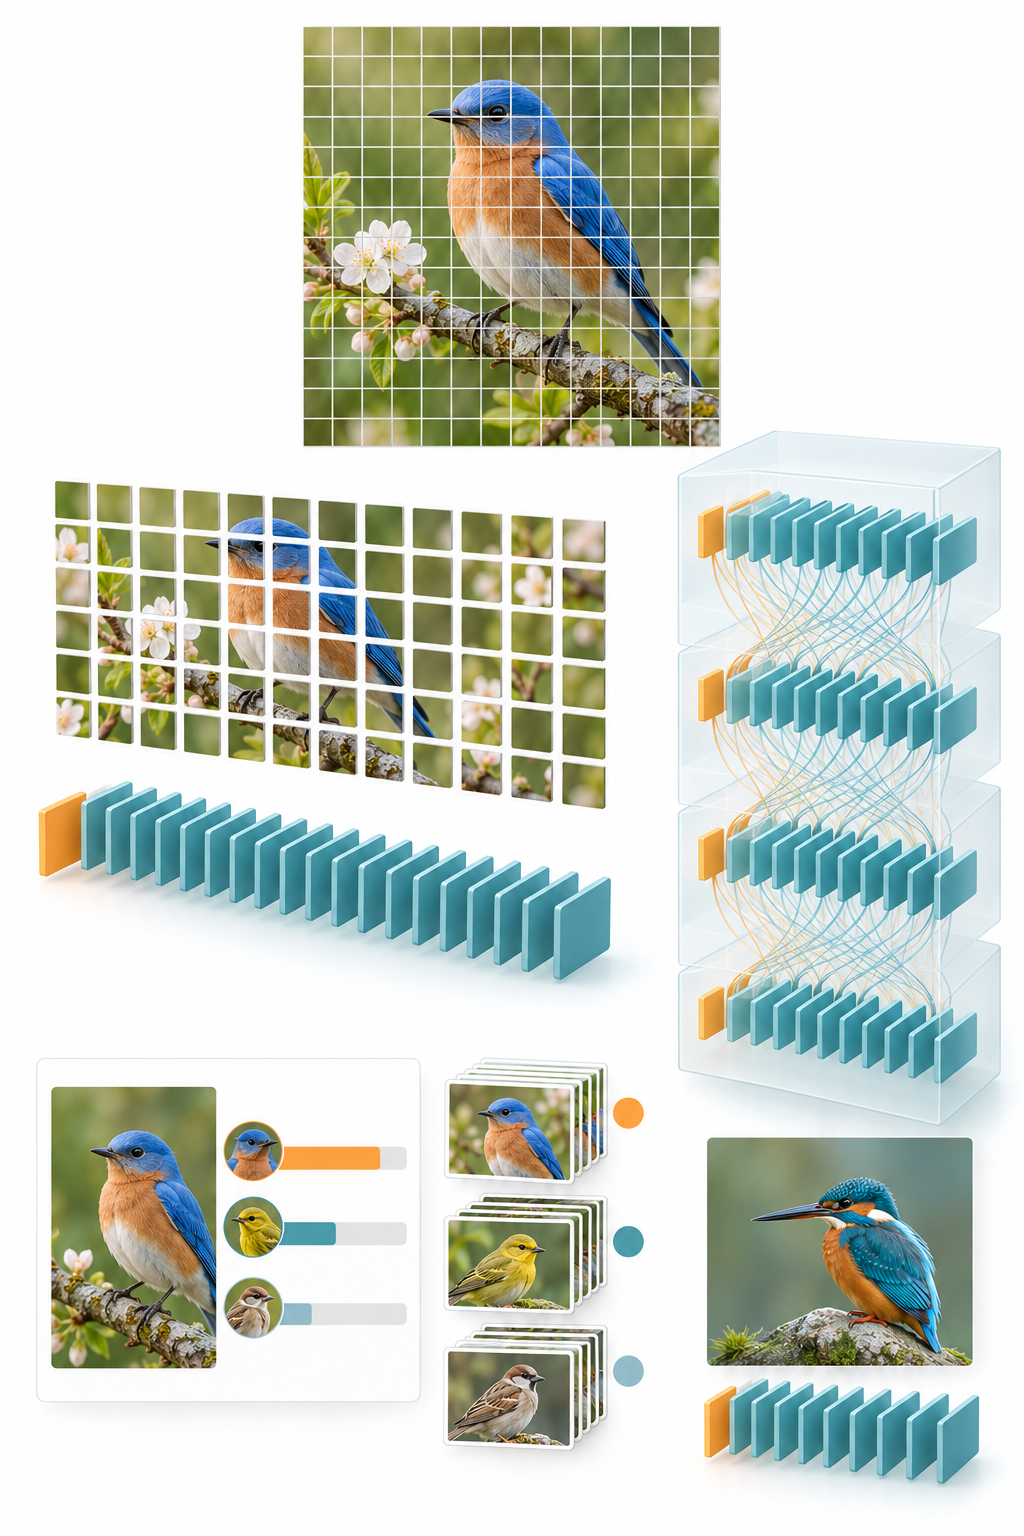
\includegraphics[width=26mm,height=31mm,keepaspectratio,viewport=30 936 990 1516,clip]{vit-imagegen-draft.png}};
\draw[-{Latex[length=2mm]},teal,line width=.7pt] (52.5,190.5) -- (52.5,187);
\fill[pale,rounded corners=2mm] (1,145) rectangle (104,186);
\node[anchor=north west,text=teal,font=\bfseries\fontsize{12}{15}\selectfont] at (4,184) {B 编码器 · §3.1 / 附录 A};
\node[anchor=north west,text width=66mm,inner sep=0] at (4,176) {ViT-B：重复 12 层\\LN $\rightarrow$ 多头注意力 + 残差\\LN $\rightarrow$ MLP + 残差\\每层输出仍为 $197\times768$};
\node[anchor=center,inner sep=0] at (88,162) {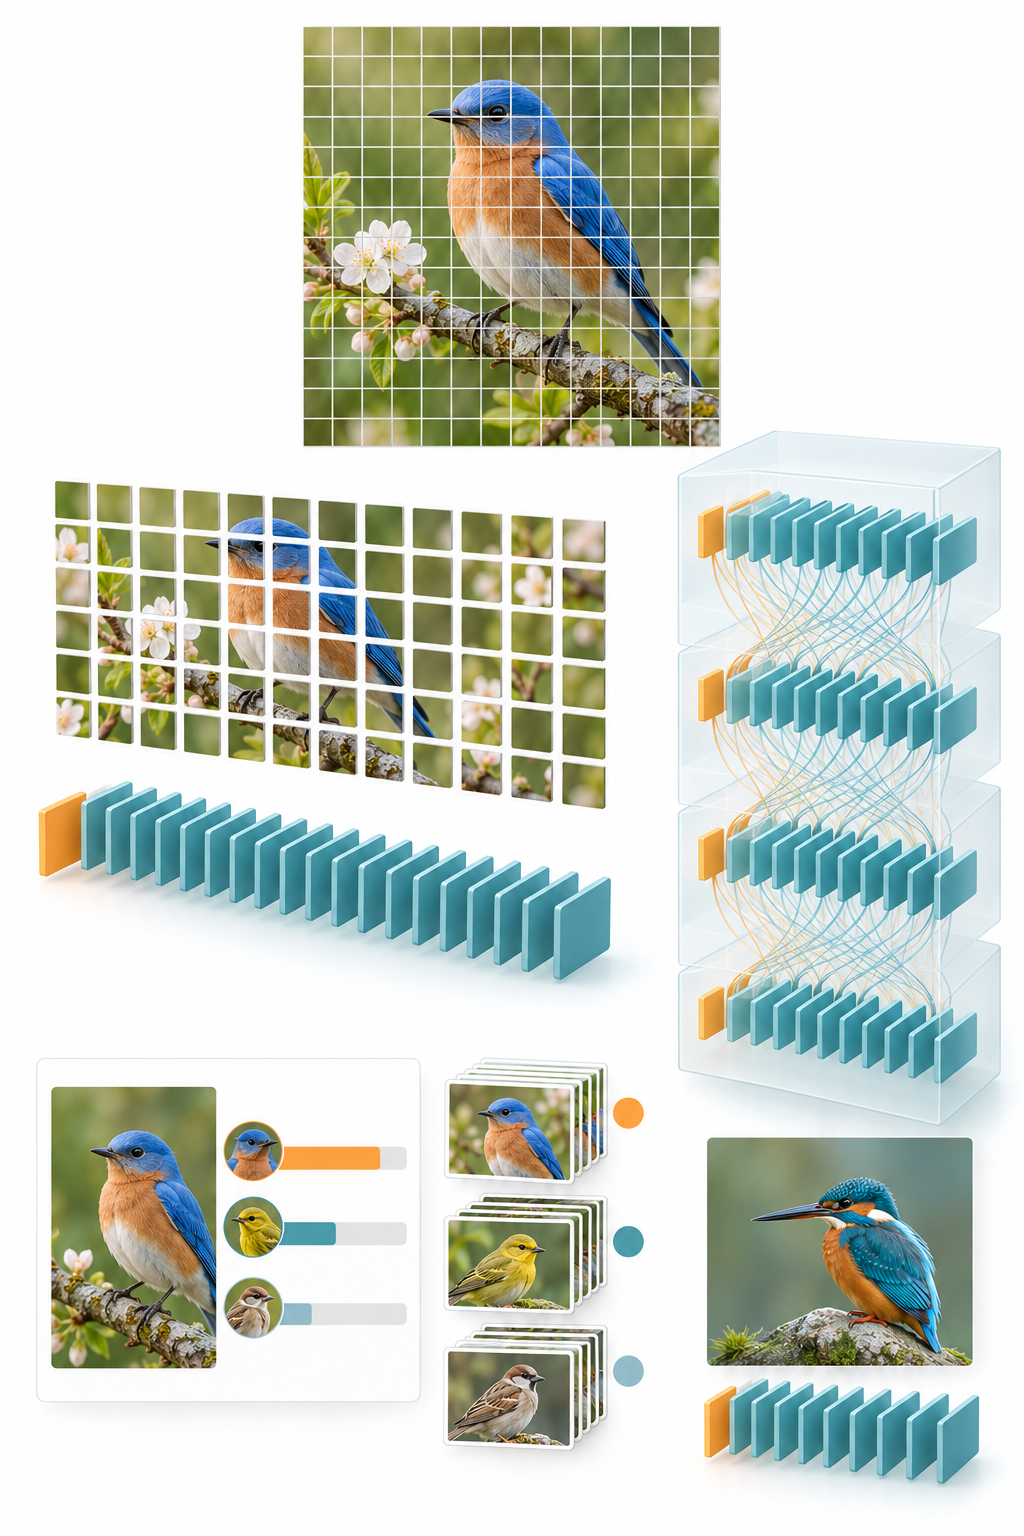
\includegraphics[width=26mm,height=31mm,keepaspectratio,viewport=655 426 1000 1006,clip]{vit-imagegen-draft.png}};
\draw[-{Latex[length=2mm]},teal,line width=.7pt] (52.5,144.5) -- (52.5,141);
\fill[pale,rounded corners=2mm] (1,99) rectangle (104,140);
\node[anchor=north west,text=teal,font=\bfseries\fontsize{12}{15}\selectfont] at (4,138) {C 分类出口 · §3.1};
\node[anchor=north west,text width=66mm,inner sep=0] at (4,130) {只取 CLS 的末层表示 $y$\\预训练：MLP 分类头\\softmax $\rightarrow$ 类别概率\\不是每个块各投一票};
\node[anchor=center,inner sep=0] at (88,116) {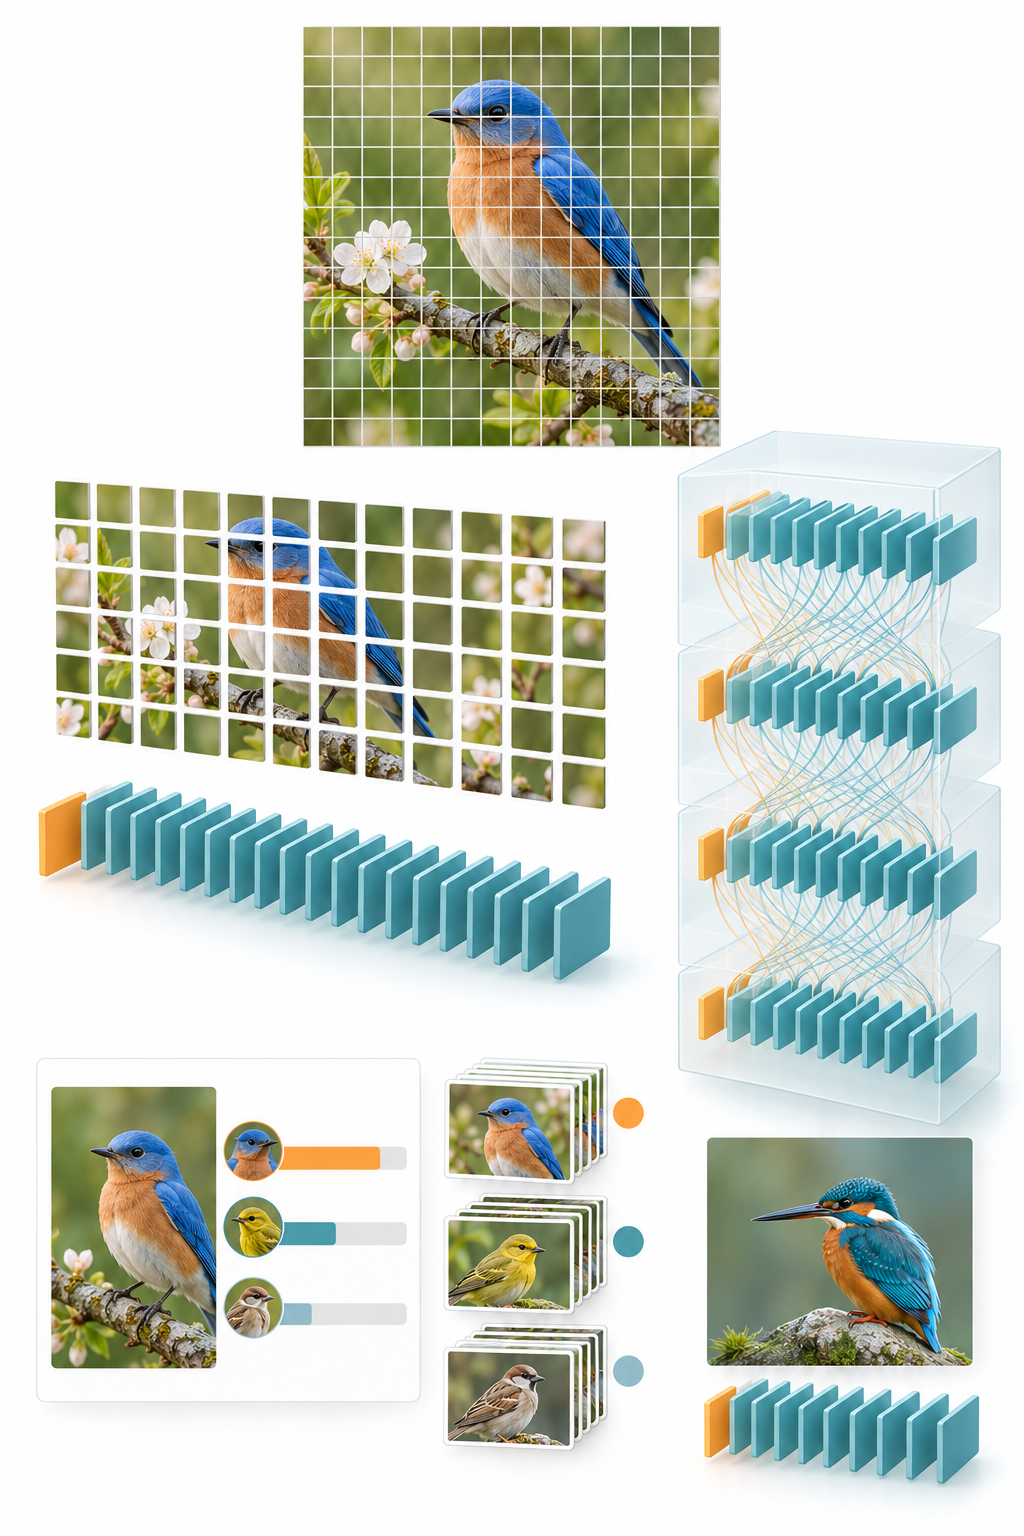
\includegraphics[width=26mm,height=31mm,keepaspectratio,viewport=20 36 430 436,clip]{vit-imagegen-draft.png}};
\draw[-{Latex[length=2mm]},teal,line width=.7pt] (52.5,98.5) -- (52.5,95);
\fill[warm,rounded corners=2mm] (1,53) rectangle (104,94);
\node[anchor=north west,text=teal,font=\bfseries\fontsize{12}{15}\selectfont] at (4,92) {D 标签怎样教它 · §4.1};
\node[anchor=north west,text width=66mm,inner sep=0] at (4,84) {训练图像与标签 $c$\\$\mathcal L=-\log p_c$\\梯度更新编码器和分类头\\大量数据补足视觉先验};
\node[anchor=center,inner sep=0] at (88,70) {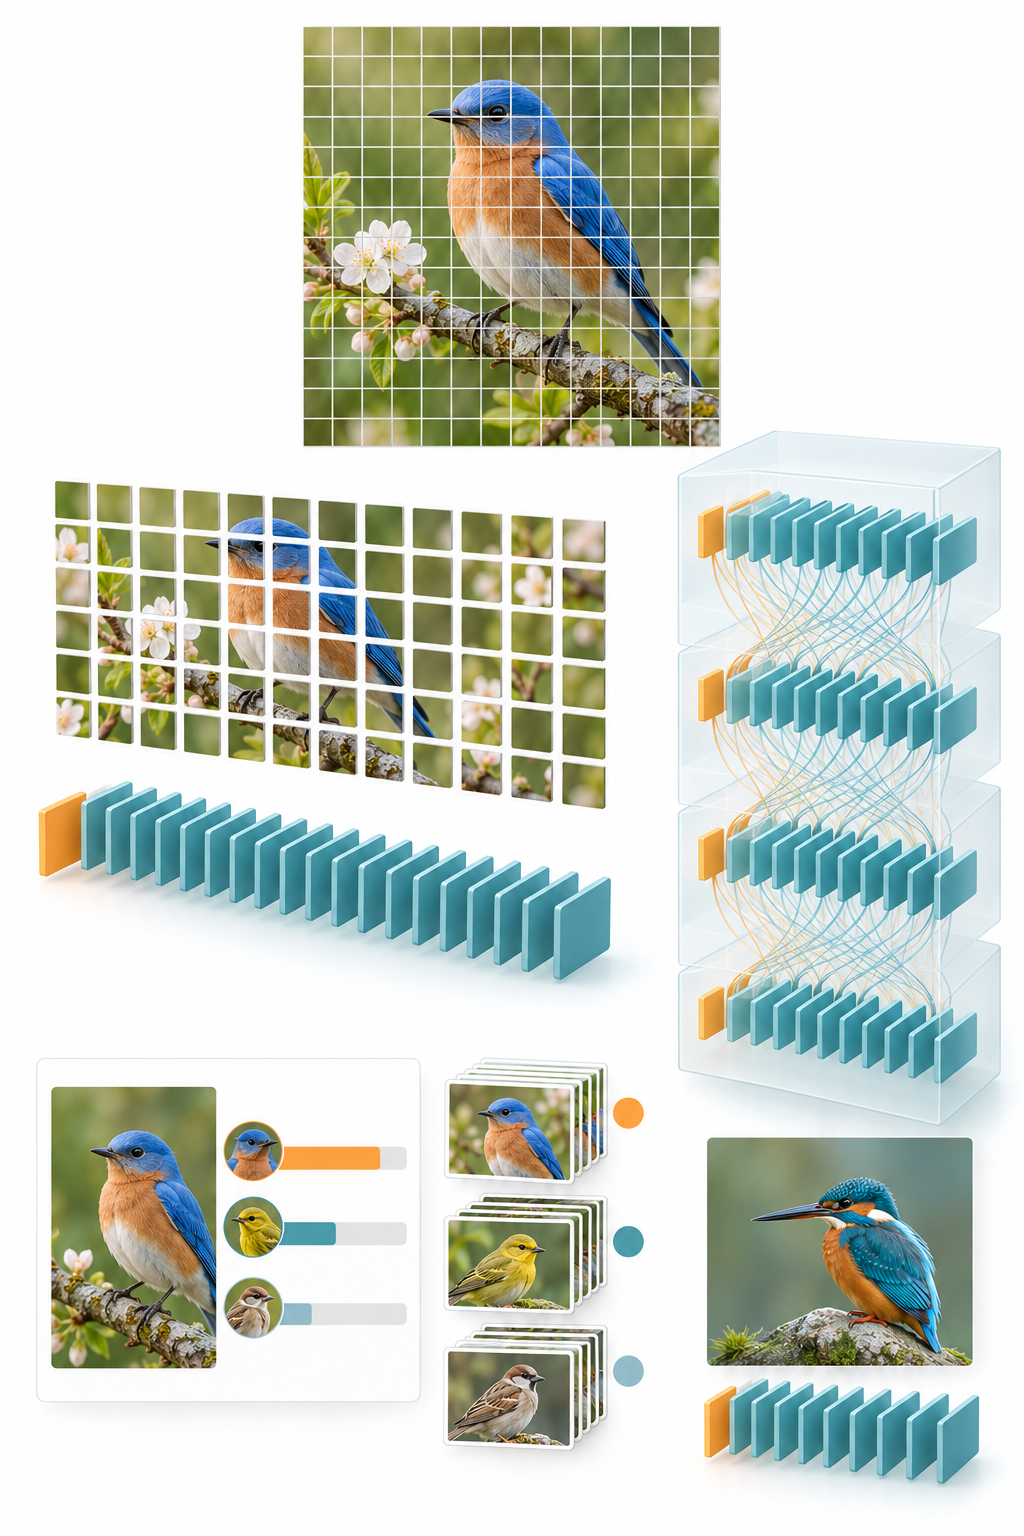
\includegraphics[width=26mm,height=31mm,keepaspectratio,viewport=390 26 700 406,clip]{vit-imagegen-draft.png}};
\draw[-{Latex[length=2mm]},teal,line width=.7pt] (52.5,52.5) -- (52.5,49);
\fill[pale,rounded corners=2mm] (1,7) rectangle (104,48);
\node[anchor=north west,text=teal,font=\bfseries\fontsize{12}{15}\selectfont] at (4,46) {E 换任务 / 更清楚的图 · §3.2};
\node[anchor=north west,text width=66mm,inner sep=0] at (4,38) {换新分类头，整体微调\\$224\rightarrow384$：$196\rightarrow576$ 块\\位置编码做二维插值\\§4 比较数据规模与算力};
\node[anchor=center,inner sep=0] at (88,24) {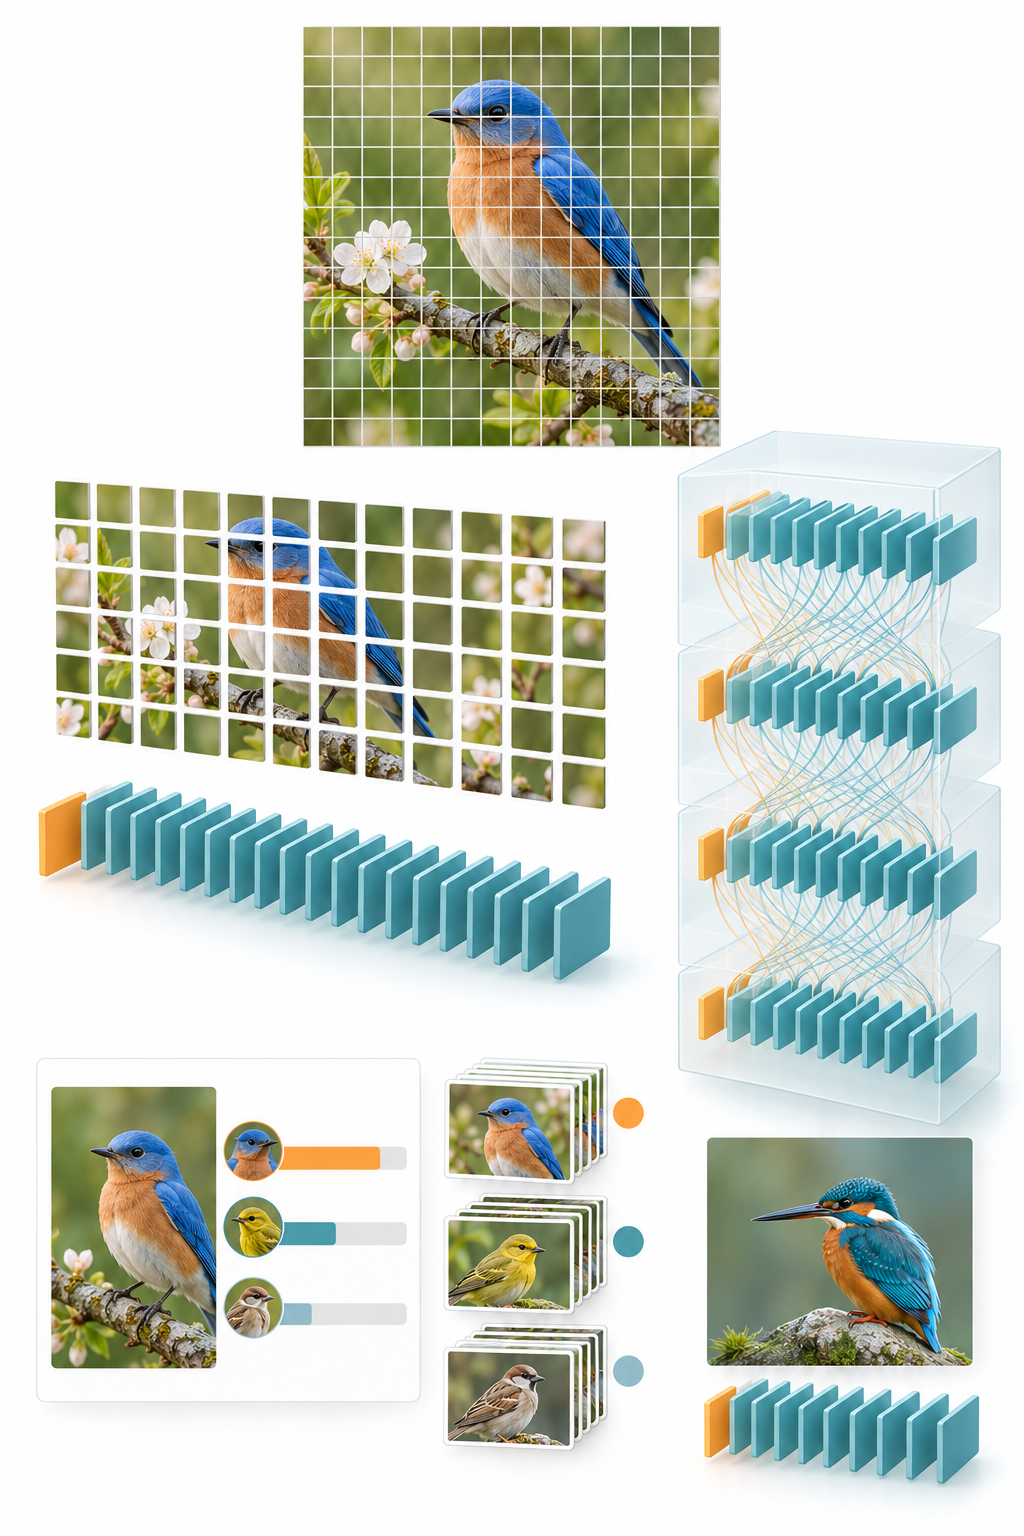
\includegraphics[width=26mm,height=31mm,keepaspectratio,viewport=690 16 1010 406,clip]{vit-imagegen-draft.png}};
\end{tikzpicture}\end{document}